To numerically solve a set of PDEs, iterative methods are frequently used to approximate the solution by a step by step phenomena. Thus, the continuous time and space domains are discretized so that a set of numerical computations are iteratively (time discretization) applied on a mesh (space discretization). In other words, the PDEs are transformed to a set of numerical computations applied at each time step on all elements of the discretized space domain. Among the numerical computations is found a set of numerical schemes, also called \textit{stencil computations}.
A formal definition of a \textit{stencil program}, and the parallelization of such program, are presented in this section.

%-------------------------------------
\subsection{Definitions}

A mesh $\mathcal{M}$ defines the discretization of the continuous space domain $\Omega$ of a set of PDEs and is defined as followed. 

\begin{mydef}
\textit{A mesh is a connected undirected graph $\mathcal{M}=(V,E)$, where $V$ is the set of vertices and $E$ the set of edges. The set of edges $E$ of a mesh $\mathcal{M}=(V,E)$ does not contain bridges.}
\end{mydef}

\begin{mydef}
$D_i$ is a set of elements of a mesh $\mathcal{M}=(V,E)$, constructed by a function $domain_i$ which defines a precise association between $V$ and $E$, $domain_i : V \times E \rightarrow D_i$.
\end{mydef}
For example, the set of cells $D_0$ in a Cartesian 2D mesh could be defined by exactly four vertices and four edges connected as a cycle. But we could also define another set of elements $D_1$ as the simple set of vertices $V$ etc.

A mesh can be structured (as Cartesian or curvilinear meshes), unstructured, regular or irregular (without the same topology for each element) and hybrid. 

\begin{figure}[!h]\begin{center}
  \resizebox{8cm}{!}{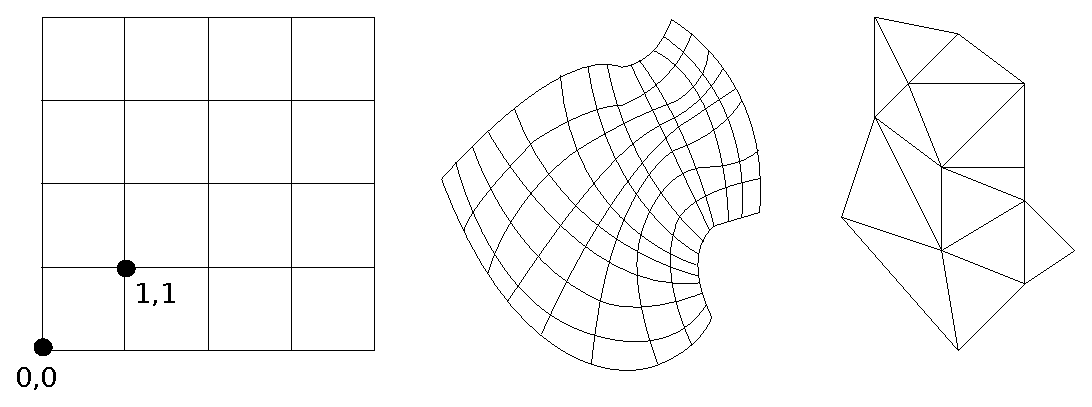
\includegraphics{./images/maillages.pdf}}
  \caption{From left to right, Cartesian, curvilinear and unstructured meshes.}
  \label{fig:mesh}
\end{center}\end{figure}

\begin{mydef}
The discretization of the continuous time domain $\mathcal{T}$ is denoted $T$ such that $\forall t_i, t_{i+1} \in T, \exists \Delta t \in \mathbb{R}$, $t_{i+1} = t_i + \Delta t$. Thus, $T$ is responsible for the iteration time steps of the numerical simulation. 
\end{mydef}

In a numerical simulation a set of data, or quantities, are applied onto the mesh and represent the set of values to compute, or to use, for computation.

\begin{mydef}
The set of data applied on the mesh is denoted by $\Delta$, such that $\delta \in \Delta$ is a function which associates each element $d \in D_i$ to a value $v \in V$, $\delta : D_i \rightarrow V$.
\end{mydef}
One can notice that in applied mathematics, the signature of $\delta$ would be $\delta : E_i \times T \rightarrow V$, however when programming a numerical simulation it is not wise to store all values of each time iteration.

\begin{mydef}
A numerical expression $\text{exp}$ is a function which represents how to compute, for an element $d \in D_i$, a data $w \in \Delta$ (written data) with a set $R \subset \Delta$ of input data (read data), $\text{exp} : R \times D_i \rightarrow w \times D_i$.
\end{mydef}

\begin{mydef}
A computation $c$ of a numerical simulation is defined as $c(R,w,D,\text{exp})$, where $R \subset \Delta, w \in \Delta$ and $\text{exp}$ a numerical expression $\text{exp} : R \rightarrow w$. $D$ is one of the subsets $D_i \subset \mathcal{M}$, such that $w : D \rightarrow V$.
\end{mydef}
It has to be noticed that at each time iteration, all the elements of a mesh are computed. However, it happens that the computation of the mesh elements is splitted in different computations (for example the computation of the physical border). In this case additional $D_i$ can be specified for the mesh $\mathcal{M}$.

\begin{mydef}
The set of $n$ ordered computations of a numerical simulation is denoted $\Gamma = [c_i]_{0 \leq i \leq n-1}$, such that $\forall c_i,c_j$ with $i \leq j$, $c_i$ is computed before $c_j$, and $c_j$ can be computed only when $c_i$ is finished.
\end{mydef}

\begin{mydef}
Finally, a \textit{multi-stencil program} is defined by the quadruplet $\mathcal{MSP}(T,\mathcal{M},\Delta,\Gamma)$.
\end{mydef}
%If the number of computations in $\Gamma$ is $card(\Gamma)=n$, such that $\bigcup_{i=0}^{n-1}c_i = \Gamma$, then $\bigcup_{i=0}^{m-1}R_i \cup w_i \subseteq \Delta$.

\begin{mydef}
The neighborhood $\mathcal{N}$ of an element $d \in D_i$ is a function to define a set of elements in any $D_k \subset \mathcal{M}$, $\mathcal{N} : D_i \rightarrow D_k \times D_k \times \dots$.
\end{mydef}
The function $\mathcal{N}$ is also sometimes called the \textit{stencil shape}, or the \textit{stencil} in applied mathematics.

A computation $c \in \Gamma$ can be of two different types. The first type is called a \textit{stencil computation}.

\begin{mydef}
A \textit{stencil computation} is defined as a quintuplet $s(R,w,D,\text{exp},\mathcal{N})$, where $R \subset \Delta, w \in \Delta$, $D$ is one the subsets $D_i$ and $w : D \rightarrow V$.
\end{mydef}
In a stencil computation $s$, $\forall d \in D$, the stencil numerical expression $\text{exp}$ is applied such that $w(d) = \text{exp}(R(d),R(\mathcal{N}(d))$. In this work, a stencil computation $s(R,w,D,\text{exp},\mathcal{N})$ always verifies $R \cap w = \emptyset$, otherwize an implicit numerical scheme has to be solve which is over the scope of this paper.

Figure~\ref{} gives an example of a stencil computation $s(R,w,D,\text{exp},\mathcal{N})$, where $\mathcal{M}(V,E)$ is a two dimensional Cartesian mesh. A single domain $D$ is defined in this example and is composed of cells formed by a cycle of four vertices $v \in V$ and four edges $e \in E$. Furthermore, in this example $R=\{A\}$, $w=B$, and for $(x,y) \in D$ the neighborhood function is 
\begin{equation*}
\mathcal{N} : (x,y) \rightarrow \{(x,y+1),(x,y-1),(x+1,y),(x-1,y)\}.
\end{equation*}
Finally, the numerical expression of this example is 
\begin{equation*}
\text{exp}(A(x,y),A(\mathcal{N}(x,y)) = B(x,y) = A(x,y)+(A(x,y+1)+A(x,y-1)+A(x+1,y)+A(x-1,y))/4.
\end{equation*}

Finally, the second type of numerical computation is a local computation.
\begin{mydef}
A local computation is a quadruplet $l(R,w,D,\text{exp})$, where $e$ does not involve a neighborhood function $\mathcal{N}$.
\end{mydef}

%-------------------------------------
\subsection{Parallelization}
\label{sect:parall}
Multi-stencil mesh-based numerical simulation can be parallelized in various ways and is an interesting kind of application to take advantage of modern heterogeneous HPC architectures, mixing clusters, multi-cores CPUs, vectorization units, GPGPU and many-core accelerators.

\paragraph{Coarse-grain data parallelism.} In a data parallelization technique, the idea is to split the data on which the program is computed in balanced sub-parts, one for each available resource. The same sequential program can afterwards be applied on each sub-part simultaneously, with some additioinal synchronizations between resources to update the data not computed locally and thus to guarantee a correct result.

More formally, the data parallelization of a multi-stencil program $\mathcal{MSP}(T,\mathcal{M},\Delta,\Gamma)$ consists in, first, a partitioning of the mesh $\mathcal{M}$ in $p$ balanced sub-meshes (for $p$ resources) $\{\mathcal{M}_0,\dots,\mathcal{M}_{n-1}\}$. This step can be performed by an external graph partitionner~\cite{} and is not adressed by this paper. As a data is mapped onto the mesh, the set of data $\Delta$ is partitionned the same way than the mesh in $\{\Delta_0,\dots,\Delta_{n-1}\}$. The second step of the parallelization is to identify in $\Gamma$ the needed synchronizations between resources to update data, and thus to build a new ordered list of computations $\Gamma'$.

\begin{mydef}
For $n$ the number of computations in $\Gamma$, and $i<j<n$, a \textit{synchronisation} is needed between $c_i$ and $c_j$, denoted $c_i \ll c_j$, if $c_j=s_j(R_j,w_j,D_j,\text{exp}_j)$, and $w_i \cap R_j \neq \emptyset$. Moreover, the data to update is $w_i \cap R_j$.
\end{mydef}

Actually, a synchronization can only be needed by the data read in a stencil computation, and only if this data has been modified before, which means that it has been written before. This synchronization is needed because the neighborhood function $\mathcal{N}$ of the stencil computation involves values computed on different resources.

\begin{mydef}
A synchronization between two computations $c_i \ll c_j$ is defined as a specific computation $\text{update}(w_i \cap R_j)$.
\end{mydef}

We denote an function to insert at a precise position of a given ordered list, a computation $c_{up}$, as
\begin{equation}
\text{insert} : [c_k]_{0 \leq k \leq n-1} \times \text{position} \times c_{up} \rightarrow [c_0,\dots,c_{\text{position}-1},c_{up},\dots,c_{n-1}]
\end{equation}

The new ordered list of computations $\Gamma'$ is obtained from the insertion of the synchronizations at the good position. Algorithm~\ref{alg:gammaprime} illustrates how $\Gamma'$ is build.
\begin{center}
\begin{algorithm}
$\Gamma' = \Gamma$\\
$\text{offset} = 0$\\
\For{$c_j \in \Gamma$}{
	\uIf{$c_j$ is a stencil}{
	\uIf{$\Gamma[c_0:c_j]==[]$}{
	$\text{insert}(\Gamma',0,\text{update}(R_j)$\\
	$\text{offset}++$\\
	}
	\uElse{
	\For{$c_i \in \Gamma[c_0:c_j]$}{
	\uIf{$c_i \ll c_j$}{
	$\text{insert}(\Gamma',j+\text{offset},\text{update}(w_i \cap R_j)$\\
	$\text{offset}++$
	}
	}
	}
	}
	}
\caption{Creation of $\Gamma'$ from $\Gamma$}
\label{alg:gammaprime}
\end{algorithm}
\end{center}

 The final step of this parallelization is to run $\Gamma'$ on each resource. Thus, for each resource $0 \leq k \leq p-1$ a multi-stencil program defined by
\begin{equation}
\mathcal{MSP}_k(T,\mathcal{M}_k,\Delta_k,\Gamma'),
\end{equation}
is runned.

We denote this parallelization technique a coarse-grain data parallelization in contrast with the same technique applied to the finer level of a single computation. In this case, for a computation $c(R,w,D,\text{exp})$, the local domain $D$ is divided for $p$ resources $\{D_0,\dots,D_{p-1}\}$, and each resource $k$ is responsible for a sub-computation $c_k(R,w,D_k,\text{exp})$.
This finer data parallelization does not require the addition of synchronizations because each computation . This finer data parallelization technique is not directly adressed by the work presented in this paper as it will be explained later. 

\paragraph{Task parallelism.}

